\documentclass[12pt, a4paper, oneside]{Thesis} % Paper size, default font size and one-sided paper
\usepackage{wrapfig}
\usepackage{lscape}
\usepackage{rotating}
\usepackage{graphicx}
\usepackage{caption}
\usepackage{amsmath}
\usepackage[utf8]{inputenc}

\usepackage{lineno}
\modulolinenumbers[5]


\usepackage{amssymb}
\usepackage{graphicx}
\usepackage{array}
\usepackage{float}
\usepackage{placeins}
\usepackage{stackengine}
\usepackage{url}
\usepackage{numprint}
\usepackage{caption}

\usepackage{booktabs}  
\usepackage{siunitx}
%\usepackage[showframe=false]{geometry}
\usepackage{subfigure}
\usepackage{hyperref}

\nprounddigits{3}
\newcolumntype{P}[1]{>{\centering\arraybackslash}p{#1}}
\newcolumntype{M}[1]{>{\centering\arraybackslash}m{#1}}

\setstackEOL{\#}
\setstackgap{L}{12pt}


%\usepackage{subcaption} %incompatible with subfig
\graphicspath{{Pictures/}} % Specifies the directory where pictures are stored

\hypersetup{urlcolor=black, colorlinks=false} % Colors hyperlinks in blue - change to black if annoyingv`	

\thesistitle{Motion Clustering Using Machine Learning}
\supervisor{Partha Pratim Das}
\degree{Bachelor of Technology}
\degreemajor{Computer Science and Engineering}
\authors{Karri Sai Satish Kumar Reddy}
\rollno{15CS10018}
\university{Indian Institute of Technology Kharagpur}
\department{Department of Computer Science and  Engineering}
\unisite{http://www.iitkgp.ac.in}
\depsite{http://www.iitkgp.ac.in/department/CS}
\placeshrt{Kharagpur}
\placelng{Kharagpur - 721302, India}
\datesub{May 03 , 2019}
\datesig{May 03 , 2019}
\semsub{Spring Semester, 2019-20}
\keywords{Steel Structure}
\coursecd{Project-II (CS47006) }

\title{\ttitle} % Defines the thesis title - don't touch this
\begin{document}
%\makeatletter
%\renewcommand*{\NAT@nmfmt}[1]{\textsc{#1}}
%\makeatother

% prints author names as small caps


\frontmatter % Use roman page numbering style (i, ii, iii, iv...) for the pre-content pages

\setstretch{1.6} % Line spacing of 1.6 (double line spacing)

% Define the page headers using the FancyHdr package and set up for one-sided printing
\fancyhead{} % Clears all page headers and footers
\rhead{\thepage} % Sets the right side header to show the page number
\lhead{} % Clears the left side page header

%\pagestyle{fancy} % Finally, use the "fancy" page style to implement the FancyHdr headers

\newcommand{\HRule}{\rule{\linewidth}{0.5mm}} % New command to make the lines in the title page

% PDF meta-data
\hypersetup{pdftitle={\ttitle}}
\hypersetup{pdfsubject=\subjectname}
\hypersetup{pdfauthor=\authornames}
\hypersetup{pdfkeywords=\keywordnames}

%----------------------------------------------------------------------------------------
%	TITLE PAGE
%----------------------------------------------------------------------------------------
\maketitle
%\titlepg % Add a gap in the Contents, for aesthetics

\clearpage % Start a new page

%----------------------------------------------------------------------------------------
%	DECLARATION PAGE
%	Your institution may give you a different text to place here
%----------------------------------------------------------------------------------------


\Declaration% Add a gap in the Contents, for aesthetics


%----------------------------------------------------------------------------------------
%	CERTIFICATE PAGE
%----------------------------------------------------------------------------------------

\addtotoc{Certificate} % Add the "Abstract" page entry to the Contents

\certificate{\addtocontents{toc}{} % Add a gap in the Contents, for aesthetics

\clearpage % Start a new page

%----------------------------------------------------------------------------------------
%	ABSTRACT PAGE
%----------------------------------------------------------------------------------------

\addtotoc{Abstract} % Add the "Abstract" page entry to the Contents

\abstract{\addtocontents{toc}{} % Add a gap in the Contents, for aesthetics

Clustering analysis has been an emerging research issue in data mining due its variety of applications.In this paper,we try to apply clustering for the domain of dance videos.We attempted to group the similar motions in a given "BharataNatyam" dance video.We have explained indetail the techniques used in our approach like optical flow,DTW and Spectral Clustering in chapter2.Then we explained our approach and concluded with the results of the approach.

}

\clearpage % Start a new page



%----------------------------------------------------------------------------------------
%	ACKNOWLEDGEMENTS
%----------------------------------------------------------------------------------------

\setstretch{1.3} % Reset the line-spacing to 1.3 for body text (if it has changed)

\acknowledgements{\addtocontents{toc}{}%\vspace{1em}} % Add a gap in the Contents, for aesthetics

I would like to express my sincere thanks to my advisor Prof.Partha Pratim Das.He was always approachable despite of his tight schedule.

I am also thankful to Himadri Buyan for helping me with a lot of valuable discussions.I express my profound thanks towards all faculty of Computer Science and Engineering department at Indian Institute of Technology, who build strong foundations for research through various courses.

Finally, I want to thank my family members and friends for their continuous support and love

}
\clearpage % Start a new page

%----------------------------------------------------------------------------------------
%	LIST OF CONTENTS/FIGURES/TABLES PAGES
%----------------------------------------------------------------------------------------

\pagestyle{fancy} % The page style headers have been "empty" all this time, now use the "fancy" headers as defined before to bring them back

\lhead{\emph{Contents}} % Set the left side page header to "Contents"
\tableofcontents % Write out the Table of Contents


%----------------------------------------------------------------------------------------
%	ABBREVIATIONS
%----------------------------------------------------------------------------------------




%----------------------------------------------------------------------------------------
%	PHYSICAL CONSTANTS/OTHER DEFINITIONS
%----------------------------------------------------------------------------------------
%
%\clearpage % Start a new page
%
%\lhead{\emph{Physical Constants}} % Set the left side page header to "Physical Constants"
%
%\listofconstants{lrcl} % Include a list of Physical Constants (a four column table)
%{
%Speed of Light & $c$ & $=$ & $2.997\ 924\ 58\times10^{8}\ \mbox{ms}^{-\mbox{s}}$ (exact)\\
%% Constant Name & Symbol & = & Constant Value (with units) \\
%}

%----------------------------------------------------------------------------------------
%	SYMBOLS
%----------------------------------------------------------------------------------------



%----------------------------------------------------------------------------------------
%	DEDICATION
%----------------------------------------------------------------------------------------
%
%\setstretch{1.3} % Return the line spacing back to 1.3
%
%\pagestyle{empty} % Page style needs to be empty for this page
%
%\dedicatory{For/Dedicated to/To my\ldots} % Dedication text
%
%\addtocontents{toc}{\vspace{2em}} % Add a gap in the Contents, for aesthetics

%----------------------------------------------------------------------------------------
%	THESIS CONTENT - CHAPTERS
%----------------------------------------------------------------------------------------

\mainmatter % Begin numeric (1,2,3...) page numbering

\pagestyle{fancy} % Return the page headers back to the "fancy" style

% Include the chapters of the thesis as separate files from the Chapters folder
% Uncomment the lines as you write the chapters

% Chapter Template

\chapter{Introduction} % Main chapter title

\label{Chapter 1} % Change X to a consecutive number; for referencing this chapter elsewhere, use \ref{ChapterX}

\lhead{Chapter 1. \emph{Introduction}} % Change X to a consecutive number; this is for the header on each page - perhaps a shortened title

%----------------------------------------------------------------------------------------
%	SECTION 1
%---------------------------------------------------------------------------------------
\section{Clustering}
Clustering analysis  has been an  emerging  research  issue in data mining due its variety of  applications.Clustering is the task of dividing data points into a number of groups such that data points in the same groups are more similar to other data points in the same group than those in other groups. In simple words, the aim is to segregate groups with similar traits and assign them into clusters. 

Clustering is  used in many fields like Market research,Biology,Search result grouping,Analysis of antimicrobial activity,Human genetic clustering etc.We are trying to use clustering to group similar motion segments in dance videos.In particular,we have clustered the \textbf{BharataNatyam} natta videos.


With the advent of many data clustering  algorithms  in  the  recent  few  years  and its extensive  use in  wide variety of applications,  including image processing, computational biology, mobile communication, medicine and economics,  has  lead  to  the  popularity of  this  algorithms.Main  problem with  the data clustering algorithms is   that it  cannot  be  standardized.   Algorithm developed may  give  best  result  with one type of data set  but  may  fail or  give  poor  result with  data set of other types.  Although  there  has  been  many  attempts   for  standardizing  the  algorithms  which can   perform   well   in  all  case  of scenarios but  till  now  no major accomplishment  has been achieved.

Many clustering algorithms  have  been  proposed so far. However, each  algorithm has its own  merits and demerits  and cannot  work  for  all  real  situations.So,we have looked into different clustering algorithms and found that \textbf{Spectral Clustering}  suits our purpose well.We have explained spectral clustering in the coming chapters.

\section{Motion Representation \& Similarity Measure}

The problem of clustering in the domain of dance is difficult compared to other domains because there was no fixed representation for the dance motions.we have used \textbf{optical flow} to represent each motion as a feature vector.Since each motion spans different no of frames,the size of feature vector is different for different motions.

In clustering,for deciding whether two motions should go to same cluster or different clusters,we should have a measure to compare two motions.Each motion spans across different no of frames even the similar ones(for example motion1 may span 10 frames while motion2 may frame 15 frames).Depending on the frame rate,even the similar motions may have different frames.Hence we need to design a similarity measure to compare different sized feature vectors corresponding to each motion.

The similarity measure should be more for similar motions and less for different motions and it should be able to compare motions with different no of frames.In this report,we proposed a measure which deals with all these problems and giving a good accuracy.






\section{Problem Statement}

The goal of this research is to effectively represent motions and design a similarity measure to cluster the motions of the given \textbf{BharataNatyam} dance videos.Specifically we have tested our approach on bharatanatyam second Adavu \textbf{Natta}.The input given was a set of videos where a dancer will be performing a Natta and a motion annotation file representing the motion frame details in the video.

\section{DataSet}

The domain we are dealing is Indian Bharatanatyam. Adavu’s are the ba-
sic units of Bharatanatyam. While performing Adavu’s, the dancer stamps,
rubs, touches, slides on the ground in different ways in synchronization with the music.There are 15 Adavus in which \textbf{Natta} is the second one which we are dealing.In Natta,there are again 8 variations.

For each variation, there are 9 sets of data corresponding to 9 dancers, each set has a video and an RGB image, a skeleton image, a depth image and a mat file containing information of skeleton image for each frame in the video as shown in the fig 3.

\begin{figure} [!htbp]
\centering    
\subfigure[RGB Image]{\label{RGB Image}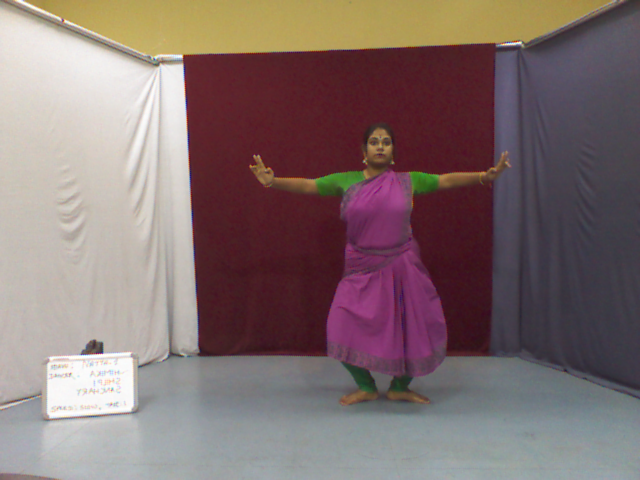
\includegraphics[width=42mm]{rgb.png}}
\subfigure[Depth Image]{\label{Depth Image}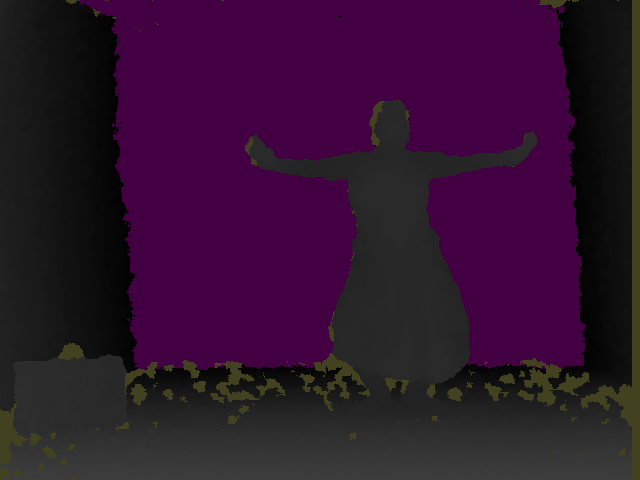
\includegraphics[width=42mm]{depth.png}}
\subfigure[Skeleton Image]{\label{Skeleton Image}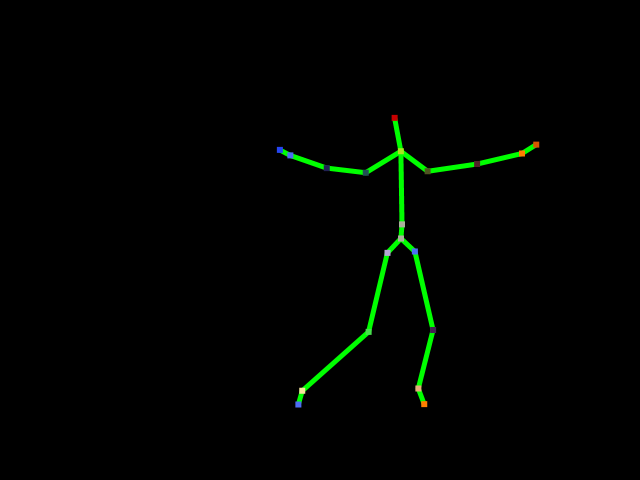
\includegraphics[width=42mm]{skeleton.png}}
\caption{Different Channels for each frame in video}
\end{figure}


In this semester,we have worked on clustering of motions using RGB image dataset.The following picture shows the scale of the data we worked on.



\begin{figure} [!htbp]
\centering
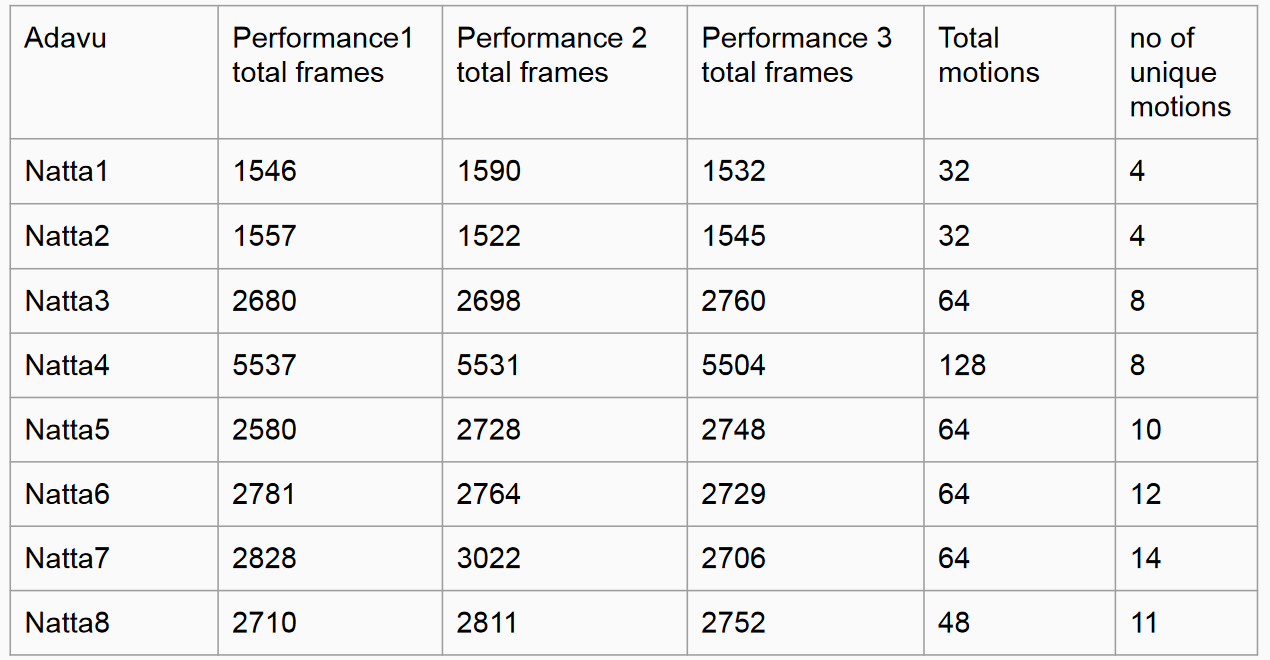
\includegraphics[width=120mm]{Pictures/data.png}
\caption{Picture showing our DataSet}
\end{figure}


Along with these videos,we also have a motion annotation file with each video consisting of motion start and end frame details for each motion in the video.  

\section{Organization of this Report}

Chapter 2 introduces the various techniques used in our approach.we explained the optical flow which we used it to represent motions in our scenario.we also explained the Dynamic Time Warping which is used as the similarity measure and then the Spectral Clustering.

In Chapter 3,we have outlined the approach we followed and the results we obtained on the mentioned dataset and discussed some insights on the results.Finally ,the conclusions will be summarized and the evaluation measure will described.Also possible areas for future work are stated briefly.
% Chapter Template

\chapter{Background, Definitions} % Main chapter title

\label{Chapter2} % Change X to a consecutive number; for referencing this chapter elsewhere, use \ref{ChapterX}

\lhead{Chapter 2. \emph{Background, Definitions}} % Change X to a consecutive number; this is for the header on each page - perhaps a shortened title

In  this  chapter,  we  provide  the  reader  with  some  material  on  the domain  of  our research  work.  A  description  of  the  methods,  algorithms  and  theoretical  features that one involved in this domain will give the reader a better understanding  of the current work. 

\section{Related Work}
In the past two decades, motion capture systems were able to track and record human motion with high spatial and temporal resolution.
The extensive proliferation of motion databases urges the development of efficient techniques to index and build models of human motion. One key aspect to understand and build better models of human motion is to develop unsupervised algorithms for decomposing human motion into a set of actions and cluster those actions.

Feng Zhou\cite{Aligned} proposed Aligned Cluster Analysis (ACA), an extension of kernel k-means clustering that allows unsupervised clustering of temporal patterns and they worked on motion capture data. Hongbin Wang,Hua Lin\cite{Spectral} provide a novel spectral clustering approach to segment multiple moving objects.But they haven't attemped for clustering.There are very few papers on this field hence we attempted to solve this particular clustering problem.Also,the available papers have only attempted to cluster using the trajectory of the motions.Hence they worked with the motion capture data.But we attempted to solve the problem using RGB videos.   



\section{Optical flow and Motion}

Optical flow is the pattern of apparent motion of image objects between two consecutive frames caused by the movement of object or camera. It is 2D vector field where each vector is a displacement vector showing the movement of points from first frame to second.Optical flow has many applications in areas like Motion estimation and video compression.Consider the image below.It shows a ball moving in 5 consecutive frames. The arrow shows its displacement vector.

\begin{figure} [!htbp]
\centering
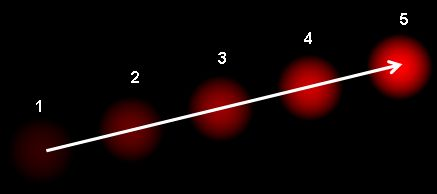
\includegraphics[width=80mm]{Pictures/opticflow.jpg}
\caption{Arrow showing optical flow}
\end{figure}



Optical flow works on several assumptions:
\begin{enumerate}
    \item The pixel intensities of an object do not change between consecutive frames.
    \item The motion between consecutive frames is small. 
    \item Neighbouring pixels have similar motion.
\end{enumerate}

Consider a pixel $I(x,y,t)$  in first frame.It moves by distance ($dx,dy$) in next frame taken after $dt$ time. So since those pixels are the same and intensity does not change, we can say, 

\[I(x,y,t)=I(x+dx,y+dy,t+dt)\]
Then taking taylor series approximation of right-hand side and neglecting higher order terms 


\[I(x,y,t) =I(x,y,t)+\frac{\partial I}{\partial x}dx+\frac{\partial I}{\partial y}dy+\frac{\partial I}{\partial t}dt \] 

\[\frac{\partial I}{\partial x}dx+\frac{\partial I}{\partial y}dy+\frac{\partial I}{\partial t}dt = 0 \]

Dividing by \(dt\) we get 
\begin{equation} \label{eq1}
f_{x}u+f_{y}v+f_{t}=0
\end{equation}

where 
    \[f_{x}=\frac{\partial f}{\partial x} \quad f_{y}=\frac{\partial f}{\partial y} \quad u=\frac{dx}{dt}\quad v=\frac{dy}{dt}\]

Above equation is called Optical Flow equation. In it, we can find \(f_{x}\) and \(f_{y}\), they are image gradients. Similarly \(f_{t}\) is the gradient along time. But ($u,v$) is unknown. We cannot solve this one equation with two unknown variables. So several methods are provided to solve this problem and one of them is Lucas-Kanade.


\subsection{Lucas-Kanade method}
We have seen an assumption before, that all the neighbouring pixels will have similar motion. Lucas-Kanade method takes a 3x3 patch around the point. So all the 9 points have the same motion. We can find $(f_{x},f_{y},f_{t})$ for these 9 points. So now our problem becomes solving 9 equations with two unknown variables which is over-determined.Those 9 equations are represented in a matrix and using the concept of psuedo inverse as shown below.

\begin{align*}
    AU = F\\
    A^{T}AU = A^{T}F\\
    U = (A^{T}A)^{-1}A^{T}F\\
\end{align*}
where
\[
A = \begin{bmatrix}
f_{x1} & f_{y1} \\
f_{x2} & f_{y2} \\
\vdots & \vdots \\
f_{x9} & f_{y9} 

\end{bmatrix} \quad
U = \begin{bmatrix}
u\\
v
\end{bmatrix} \quad
F = \begin{bmatrix}
-f_{t1}\\
-f_{t2}\\
\vdots\\
-f_{t9}
\end{bmatrix}
\]
Below is the final solution which is two equation-two unknown problem and solve to get the solution.
\[
\begin{bmatrix}
u \\ v \end{bmatrix} = \begin{bmatrix} \sum_{i}{f_{x_i}}^2 & \sum_{i}{f_{x_i} f_{y_i} } \\ \sum_{i}{f_{x_i} f_{y_i}} & \sum_{i}{f_{y_i}}^2 \end{bmatrix}^{-1} \begin{bmatrix} - \sum_{i}{f_{x_i} f_{t_i}} \\ - \sum_{i}{f_{y_i} f_{t_i}} \end{bmatrix}\]


The good thing was this was all already implemented in \textbf{open cv}.Finally note that this derivation is valid only for detecting small motions.For our purpose,the motion between two consecutive frames is very less.Hence this method can be safely applied.If we obtain ($u,v$) for every pixel in the image,then it is called dense optical flow and we have used dense optical flow in the proposed approach.

There are several other algorithms proposed to solve optical flow.you can refer them here\cite{Optical}


\section{Histogram of Optical flow}
A feature descriptor is a representation of an image or an image patch that simplifies the image by extracting useful information and throwing away extraneous information.Typically, a feature descriptor converts an image of size width x height x 3 (channels) to a feature vector / array of length n.Histogram of Optical Flow (HOF) is one such descriptor.In the case of the HOG feature descriptor, the input image is of size $h * w * 3$ and the output feature vector is of length $ h * w * 9 / 64 $.

In the HOF feature descriptor, the distribution ( histograms ) of directions of optical flow are used as features.Since, we are trying to cluster motions,optical flow serves as good feature for capturing motion.The following shows the steps in the calculation of HOF descriptor.

\textbf{Step 1 : Calculate Optical Flow}

To calculate a HOF descriptor, we need to first calculate the optical flow; after all, we want to calculate the histogram of optical flow.To calculate the optical flow, use the methods described above.Now we get two components ($u,v$) foe every pixel by using the optical flow.

\textbf{Step 2 : Calculate Histogram of Gradients in \begin{math}8*8\end{math} cells}

In this step, the image is divided into \begin{math}8*8\end{math} cells and a histogram of optical flow is calculated for each \begin{math}8*8\end{math} cells.One of the important reasons to use a feature descriptor to describe a patch of an image is that it provides a compact representation.

An \begin{math}8*8\end{math} image patch contains \begin{math}8*8*3\end{math} = 192 pixel values. The optical flow of this patch contains 2 values ( magnitude and direction ) per pixel which adds up to \begin{math}8*8*2\end{math} = 128 numbers. By the end of this section we will see how these 128 numbers are represented using a 9-bin histogram which can be stored as an array of 9 numbers. Not only is the representation more compact,calculating a histogram over a patch makes this representation more robust to noise. Individual optical flow may have noise, but a histogram over \begin{math}8*8\end{math} patch makes the representation much less sensitive to noise.

The histogram is essentially a vector ( or an array ) of 18 bins ( numbers ).First convert the optical flow ($u,v$) of every pixel into polar coordinates.The bins can be made using following two techniques

\textbf{Interval Binning}


In this technique, the bins are considered as intervals 0 - 20 , 20 - 40 ... , 340 - 360. For every pixel in the \begin{math}8*8\end{math} patch a bin is selected based on the direction, and the vote ( the value that goes into the bin ) is selected based on the magnitude.

\newpage

\textbf{Weighted Binning}

In this technique, The histogram contains 18 bins corresponding to angles 0, 20, 40 … 160. For every pixel in the \begin{math}8*8\end{math}. Depending on the direction, the magnitude is split across at most two bins depending on the distance of direction from bin angle.An illustration of this is shown below.

\begin{figure} [!htbp]
\centering
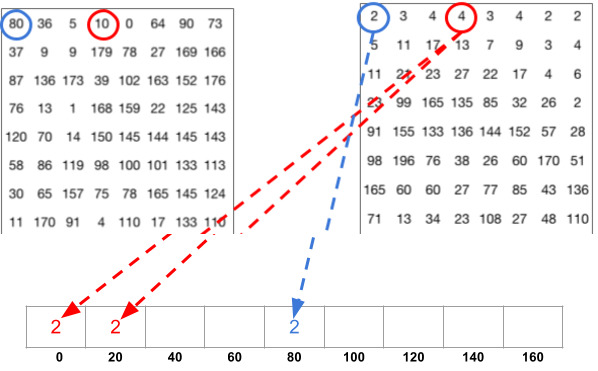
\includegraphics[width=80mm]{Pictures/HOF.jpg}
\caption{Weighted Binning illustration}
\end{figure}

Let’s first focus on the pixel encircled in blue. It has an angle ( direction ) of 80 degrees and magnitude of 2. So it adds 2 to the 5th bin. The optical flow at the pixel encircled using red has an angle of 10 degrees and magnitude of 4. Since 10 degrees is half way between 0 and 20, the vote by the pixel splits evenly into the two bins.

\textbf{Step 4 : \begin{math}16*16\end{math} Block Normalization}

In order the descriptor to be independent of lighting variations, we would like to “normalize” the histogram so they are not affected by lighting variations.A \begin{math}16*16\end{math} block has 4 histograms which can be concatenated to form a \begin{math}36 * 1\end{math} element vector and it will be normalized.The window is then moved by 8 pixels and a normalized \begin{math}36 * 1\end{math} vector is calculated over this window and the process is repeated.After doing this,all the bins are concatenated to form the final feature vector. 

But for our motion clustering, this step didn't worked well(Accuracy without this step was good).Hence we just didn't up to step 3.Let us say for each frame the HOF vector is of size x. If a motion has f frames the feature vector size will be of size $f*x$. Since it depends on number of frames,feature vector for each motion may not be of same size.










\section{Dynamic Time Warping (DTW) }

The distance between two point \({x}=[x_{1}, x_{2}, ..., x_{n}]\) and \({y}=[y_{1}, y_{2}, ..., y_{n}]\) in a n-dimensional space can be computed via the Euclidean distance: 
\[dist(\mathbf{x},\mathbf{y})=\|\mathbf{x}-\mathbf{y}\|=\sqrt{(x_1-y_1)^2+(x_2-y_2)^2+\cdots+(x_n-y_n)^2}.\]

However, if the length of \(\mathbf{x}\) is different from \(\mathbf{y}\), then we cannot use the above formula to compute the distance. Instead, we need a more flexible method that can find the best mapping from elements in \(\mathbf{x}\) to those in \(\mathbf{y}\) in order to compute the distance.

The goal of \textbf{dynamic time warping} (DTW for short) is to find the best mapping with the minimum distance by the use of DP. The method is called \textbf{"time warping"} since both x and y are usually vectors of time series and we need to compress or expand in time in order to find the best mapping.

Let t and r be two vectors of lengths m and n, respectively. The goal of DTW is to find a mapping path \( \{(p_1, q_1), (p_2, q_2), ..., (p_k, q_k)\} \)  such that the distance on this mapping path \textbf{\( \sum_{i=1}^k |t(p_i)-r(q_i)|\)} is minimized, with the following constraint:
\begin{itemize}
    \item The ordering should be preserved meaning if i is mapped with j then i-1 can be mapped with any index until j but not beyond j.This local constraint guarantees that the mapping path is monotonically non-decreasing in its first and second arguments. Moreover, for any given element in t, we should be able to find at least one corresponding element in r, and vice versa.  
\end{itemize}

\begin{figure} [!htbp]
\centering
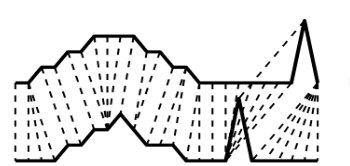
\includegraphics[width=80mm]{Pictures/dtw.png}
\caption{Figure showing the mapping obtained by DTW}
\end{figure}


\subsection{Solving DTW}

we can solve it using the following dynamic programming(DP) approach.

\begin{enumerate}
    \item \textbf{Optimum-value function} : Define $D(i,j)$ as the DTW distance between $t(1:i)$ and $r(1:j)$, with the mapping path starting from $(1,1)$ to $(i,j)$
    
    \item \textbf{Recursion} :
    \[D(i, j)=|t(i) - r(j)| + min \left\{\begin{matrix} D(i-1, j)\\D(i-1, j-1)\\D(i, j-1) \end{matrix}\right\},\]
    
     with the initial condition \(D(1, 1)=|t(1)-r(1)|\)
    \item \textbf{Final answer} : $D(m,n)$
\end{enumerate}

If we want to know the optimum mapping path in addition to the minimum distance, we may want to keep the optimum fan-in of each node. Then at the end of DP, we can quickly back track to find the optimum mapping path between the two input vectors. 

There are many attempts made to make DTW run faster.you can refer \cite{DTW} to know about a faster version of DTW.

\subsection{Applications}
Dynamic time warping is mainly used in speech recognition,since speech is very sensitive for variations in time,but the technique has proved to be useful for many other applications like gesture recognition, robotics, data mining,hand writing recognition etc


For our purpose,we used DTW for measuring similarity between motions.As we stated earlier that each motion is represented by a feature vector of different sizes.Hence we use DTW to compare these unequal sized feature vectors.Everything remains same except the t,r vectors which in our case are not simple vectors but vector of vectors.This will be explained in detail in the coming chapters.

\section{Spectral Clustering}
The goal of spectral clustering is to cluster data that is connected but not necessarily compact or clustered within convex boundaries.It very often outperforms traditional clustering algorithms such as the k-means algorithm.

\begin{figure} [!htbp]
\centering
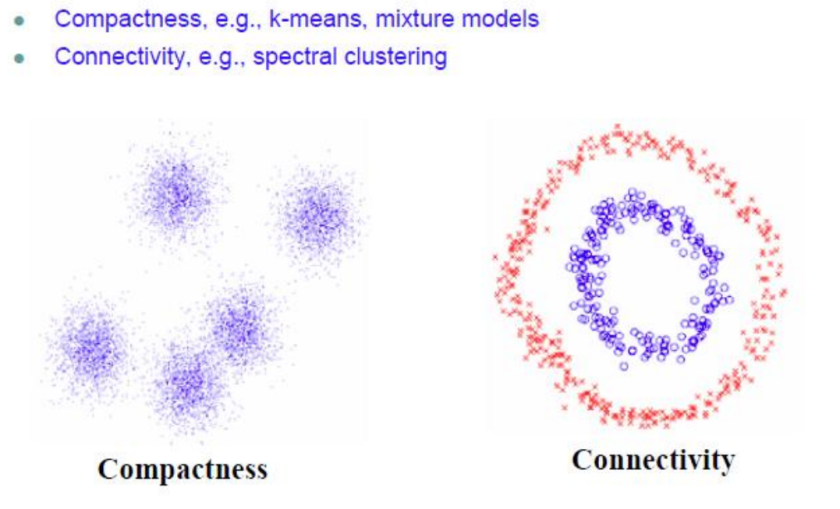
\includegraphics[width=80mm]{Pictures/spec.png}
\caption{Example explaining two properties of data}
\end{figure}

\subsection{Basic Idea}
\begin{itemize}
    \item Spectral clustering models the objective function as a graph spectrum problem and solves it with the known linear algebra techniques.
    \item It connects the objective function to one of the following  property of graph laplacian and solves it in place of minimizing objective function.
\end{itemize}

For every vector $f \in R^{n}$ we have

\[f^{'}Lf = \frac{1}{2}\sum_{i,j=1}^{n}w_{ij}\left (f_{i} - f_{j} \right )^{2}\]
where 
\[ L = D - W  , \quad \text{W is the adjacency Matrix} \]
\[d_{i} = \sum_{j=1}^{n}w_{ij} \]
\centerline{D is a diagonal Matrix with $d_{i}$  as diagonal}

\subsection{Algorithm}
\begin{enumerate}
    \item \textbf{Input} : Similarity matrix $W \in R^{n*n}$ , number k of clusters to construct
    \item Compute the unnormalized Laplacian $L$.
    \item Compute the first k eigenvectors ($u_{1},u_{2},\dots,u_{k}$) of $L$.
    \item Let $U \in R^{n*k}$ be the matrix containing the vectors $u_{1},u_{2},\dots,u_{k}$ as columns.
    \item Let $i = 1\dots n$ let $y_{i} \in R^{k}$ be be the vector corresponding to the $i_{th}$ row of U
    \item Cluster the points $(y_{i})_{i=1,\dots,n}$ in $R^{k}$ with k-means clustering algorithm into $C_{1},\dots,C_{k}$ clusters.
    \item \textbf{Output} : Clusters $A_{1},A_{2},\dots,A_{k}$ with $A_{i} = \{j | y_{i} \in C_{j} \}$
    
    
\end{enumerate}


\subsection{Objective Function}
The following is the Objective function the spectral clustering is trying to minimize
\begin{figure} [!htbp]
\centering
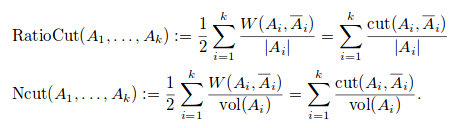
\includegraphics[width=100mm]{Pictures/obj.png}
\caption{Objective Function}
\end{figure}

Intuitively this function is trying to minimize the  sum of crossing edges between clusters while trying to maximize the within cluster edges.Note that here edge weight represent similarity.In other words,it is trying to maximize within cluster similarity while minimizing across cluster similarity.

\subsection{How the algorithm is minimizing the above Function }
This section shows how graph laplacian is related to the above objective function and hence we can minimize the laplacian property instead of that objective function.

\subsubsection{Approximating Ratio Cut for K = 2}
\begin{figure} [!htbp]
\centering
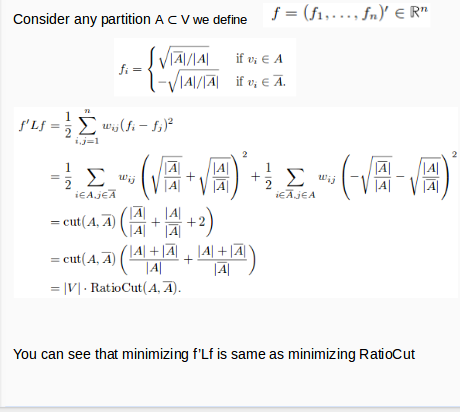
\includegraphics[width=100mm]{Pictures/k=2.png}
\caption{Figure showing how Laplacian property related to RatioCut}
\end{figure}

Finally we should minimize the below equation to minimize the objective function
\begin{figure} [!htbp]
\centering
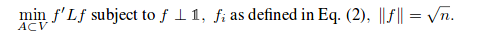
\includegraphics[width=120mm]{Pictures/minim.png}
\end{figure}

This is a discrete optimization problem but it is NP Hard.Relaxing f to take real values makes it solvable.By the Rayleigh-Ritz theorem, 
the solution to this is eigenvector corresponding to the second smallest eigenvalue of L.
\subsubsection{Approximating Ratio Cut for K \texorpdfstring{$>$}{Lg} 2}
\begin{figure}[H]
\centering
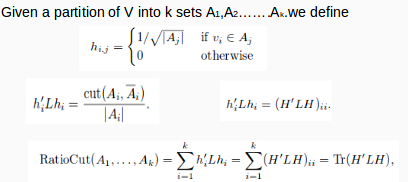
\includegraphics[width=100mm]{Pictures/k>2_half.png}
\end{figure}

The final minimization problem is
\begin{figure} [!htbp]
\centering
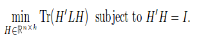
\includegraphics[width=60mm]{Pictures/spec2.png}
\end{figure}

By the Rayleigh-Ritz theorem,the solution is given by choosing H as the matrix which contains the first k eigen vectors of L as columns.So,for this reason we are calculating first k eighen vectors in the algorithm.we can refer \cite{Spectral1} for more indepth details on spectral clustering.


\section{Support Vector Machine}

A Support Vector Machine (SVM) is a supervised machine learning algorithm that can be employed for both classification and regression purposes. SVMs are more commonly used in classification problems.SVMs are based on the idea of finding a hyperplane that best divides a dataset into two classes, as shown in the image below.

\begin{figure} [!htbp]
\centering
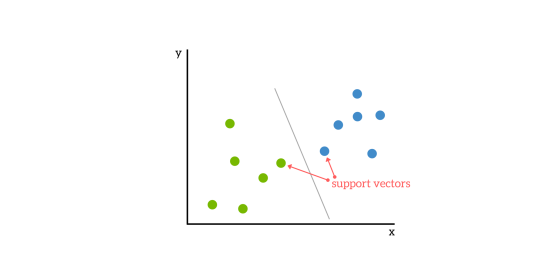
\includegraphics[width=100mm]{Pictures/svm1.png}
\caption{Figure demonstrating hyperplane}
\end{figure}

\subsection{Support Vectors}

Support vectors are the data points nearest to the hyperplane, the points of a data set that, if removed, would alter the position of the dividing hyperplane. Because of this, they can be considered the critical elements of a data set.

\subsection{HyperPlane}

As a simple example, for a classification task with only two features (like the image above), you can think of a hyperplane as a line that linearly separates and classifies a set of data.

Intuitively, the further from the hyperplane our data points lie, the more confident we are that they have been correctly classified. We therefore want our data points to be as far away from the hyperplane as possible, while still being on the correct side of it.So when new testing data is added, whatever side of the hyperplane it lands will decide the class that we assign to it.


\subsection{Finding the right hyperplane}

The distance between the hyperplane and the nearest data point from either set is known as the \textbf{margin}. The goal is to choose a hyperplane with the greatest possible margin between the hyperplane and any point within the training set, giving a greater chance of new data being classified correctly.

\begin{figure} [!htbp]
\centering
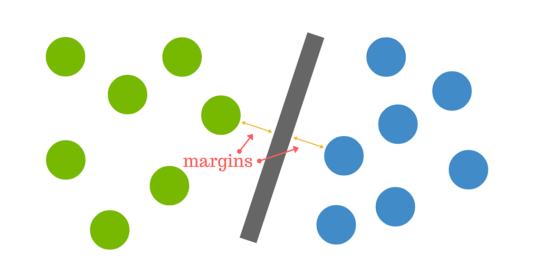
\includegraphics[width=100mm]{Pictures/svm2.png}
\caption{Figure demonstrating margin}
\end{figure}

\subsection{Linearly non separable data}

We will transform the axes and convert the data into linearly separable.The transformation of data is done using concept called \textbf{kernels}.The below figures demonstrates how the transformation is done.

\begin{figure} [!htbp]
\centering
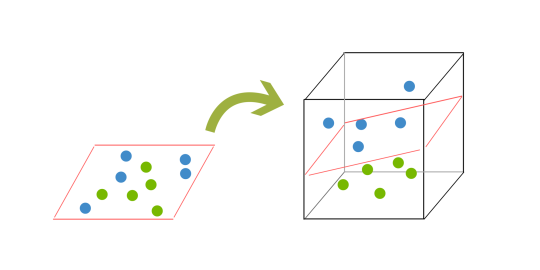
\includegraphics[width=100mm]{Pictures/svm3.png}
\caption{Figure demonstrating kernels}
\end{figure}

For mathematical foundations of SVM, refer \href{http://cs229.stanford.edu/notes/cs229-notes3.pdf}{CS229 Lecture notes}. 

\section{K- Nearest Neighbour (KNN)}

k-nearest neighbors algorithm (k-NN) is a non-parametric method used for classification and regression.In this supervised learning technique,there is no training phase.when a new data point come,it will be assigned the class of training data point which is closest to the new data point.The "closest" is defined as per application requirements.In our context the closest is defined using the measure DTW.




\section{Accuracy Measure (Rand Index)}
In order to evaluate the results obtained by our algorithm,we have used \textbf{rand index} as a evaluation measure for computing accuracy.

If C is a ground truth class assignment and K the clustering,then let:
\begin{itemize}
    \item a, the number of pairs of elements that are in the same set in C and K
    \item b, the number of pairs of elements that are in different sets in both  C and K
\end{itemize}
\[ RI = \frac{a + b}{\binom{n_{samples}}{2}}\]
















 
% Chapter Template

\chapter{Chapter3 Approach \& Results} % Main chapter title

\label{ChapterX} % Change X to a consecutive number; for referencing this chapter elsewhere, use \ref{ChapterX}

\lhead{Chapter 3. \emph{Approach \& Results}} % Change X to a consecutive number; this is for the header on each page - perhaps a shortened title
We have used both unsupervised learning and supervised learning techniques They can be explained in brief as follows:

\textbf{Unsupervised Learning}
\begin{enumerate}
    \item Used Dense optical flow and obtained the feature vector of each motion.
    \item Applied DTW  as similarity measure for motions and obtained similarity matrix.
    \item Used Spectral Clustering to cluster the data using the above similarity matrix.
\end{enumerate}

\textbf{Supervised Learning}
\begin{enumerate}
    \item Used Dense optical flow to get the features for each motion.
    \item Made all vectors equal size by appending with small value(1e-5).
    \item Used SVM for the classification.
\end{enumerate}
\section{Unsupervised Approaches}
\subsection{Feature vector for representing motions}
From the given annotation file,we know for each motion the starting and ending frame number.Let the frame corresponding to a motion be $[s,t]$.
Taking frame "s" as reference we computed dense optical flow for all the frames in the range $[s+1,t]$.

If a motion has f frames each of size 640*480
The size of feature vector will be $2*640*480*f$.The optical flow $(u,v)$ for each pixel so the 2 in the equation.Each motion feature vector can be visualized as follows:
    \[fV[1,\dots,f] , \quad \text{where f is no of frames in the motion}\]
    \[fV[i] \text{ is a 3d matrix as } V[640][480][2] \]
    
\subsection{Similarity Matrix from Feature Vectors}
These feature vectors are of different sizes because of different no of frames for each motion.So,used DTW approach to compare them.As \(fV1[i],fV2[j]\) are not simple numbers as explained in previous chapter,so, we  define  the quantity \(|fV1[i]-fV2[j]|\) as follows.

we first made \[temp[i][j] = \text{euclidean distance between } fV1[i][j][2] \text{ and } fV2[i][j][2] \] 
\[i = 1,\dots,640 \text{ and } j = 1,\dots,480 \]

And finally, 
\[|fV1[i]-fV2[j]| = \sum_{i=1}^{640}\sum_{j=1}^{380}temp[i][j]\]

Suppose there are M motions,so we define a dissimilarity matrix in this way

\[DSM[i][j] = DTW(fV[i],fV[j])\]
\[i = 1,\dots,M \text{ and } j = 1,\dots,M \]

Similarity  Matrix is obtained as 
\[ SM[i][j] = \frac{1}{DSM[i][j]} \]

\subsection{Clustering}
After obtaining similarity matrix as explained above,we tried \textbf{Affinity Propagation} and \textbf{Spectral Clustering}.In Affinity Propagation, the no of clusters best for the dataset is automatically obtained.But in case of complex nattas,the no of clusters automatically obtained is not correct.So,we left Affinity Propagation and taken Spectral Clustering.You can see the results section for more details.


\subsection{Results}
\begin{figure} [!htbp]
\centering
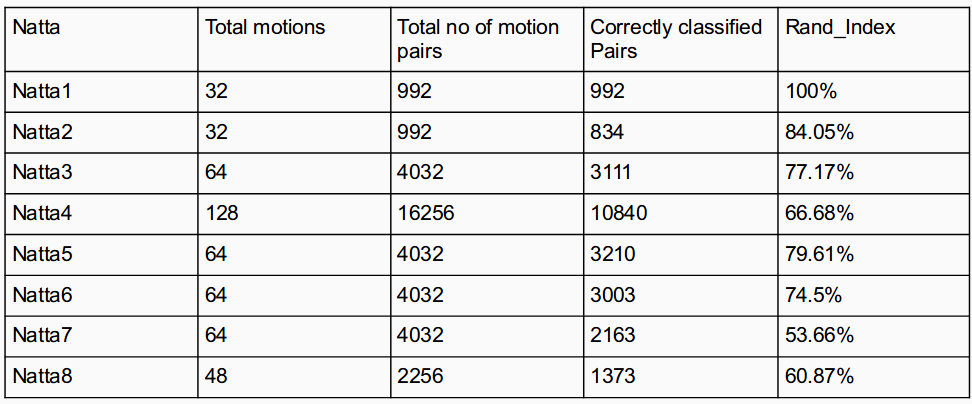
\includegraphics[width=140mm]{Pictures/res1.png}
\end{figure}


The accuracy is measured using the rand index as described in the previous chapter.We can observe the accuracy is really good for the simple motions in the initial Nattas.But as complexity of motions increases in the later nattas,the accuracy was decreased.We have analyzed reasons for less accuracy in the Analysis section.

\subsubsection{Similarity Matrix}
We can see the similarity matrix and observe the following point.Motion1 is similar with Motion5,Motion9,Motion13 which is evident by light colour in the figure.Motion0 is similar with Motion8.But because Motion4 is similar with Motion8,the Motion0,Motion4,Motion8 went into same cluster as we wanted.
\begin{figure} [H]
\centering
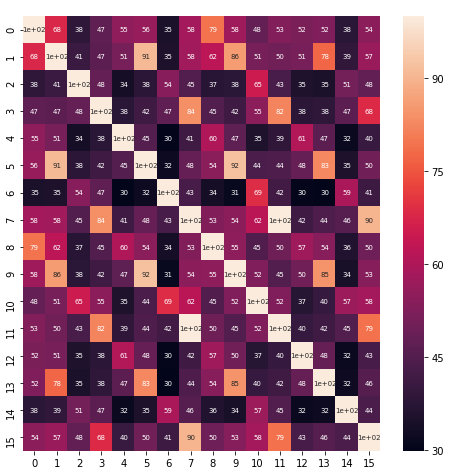
\includegraphics[width=90mm]{Pictures/sim.png}
\end{figure}
\subsubsection{Confusion Matrix}

\begin{figure} [H]
\centering
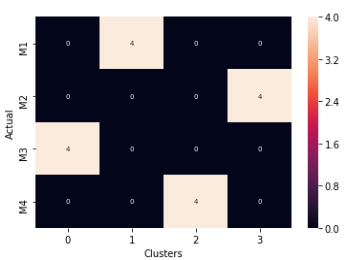
\includegraphics[width=85mm]{Pictures/confuse.png}
\end{figure}
Here you can see there are four motions of type M1 and every motion went into cluster 1.The results for other nattas and dancer can be found \href{https://docs.google.com/document/d/1tpQId7VadBUHFW8xKCehUH4VTjIplCjThj6Vl_HT_N4/edit}{here}.


\subsection{Different Variations tried}

Generally Histogram of Optical Flow is used in place of using dense optical flow directly.Hence, we tried to use HOF in place of Dense Optical Glow in the first step.Here,we tried two variations of HOF weighted binning and Interval binning.

\begin{figure} [H]
\centering
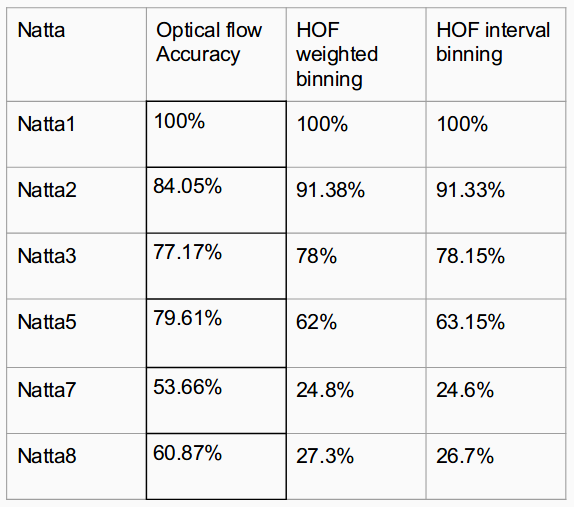
\includegraphics[width=80mm]{Pictures/res2.png}
\end{figure}

We have also tried varying binsizes to see how it affects accuracy. Increasing bin size decreases the accuracy of simple motions but increases the accuracy of complex motions.

\begin{figure} [H]
\centering
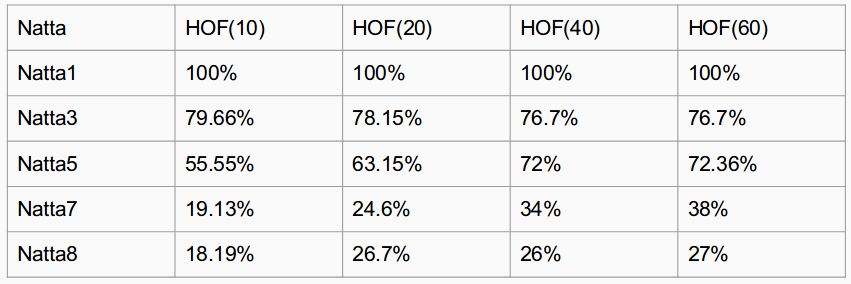
\includegraphics[width=120mm]{Pictures/res3.png}
\end{figure}

\subsection{Reasons for Low Accuracy for Natta7}

In Natta7, the number of frames for each motion differs too much.For example M1 contains 62 frames whereas M2 contains 4 frames 
Consider three motions M1,M2 and M1 in the next cycle
Since M2 has less frames DTW is assigning less cost to M1 and M2 rather than to M1 and M1 in the next cycle.So the motions with less no of frames are affecting the similarity matrix.

\textbf{Noisy Motions : } The motions having less than 10 frames are causing the accuracy to be low as explained above.Also it is highly impractical for a motion to be in such less no of frames. Hence we treat motions with less frames and removed them and recalculated accuracy for the above methods.

\subsection{Results without noisy motions}

\begin{figure} [H]
\centering
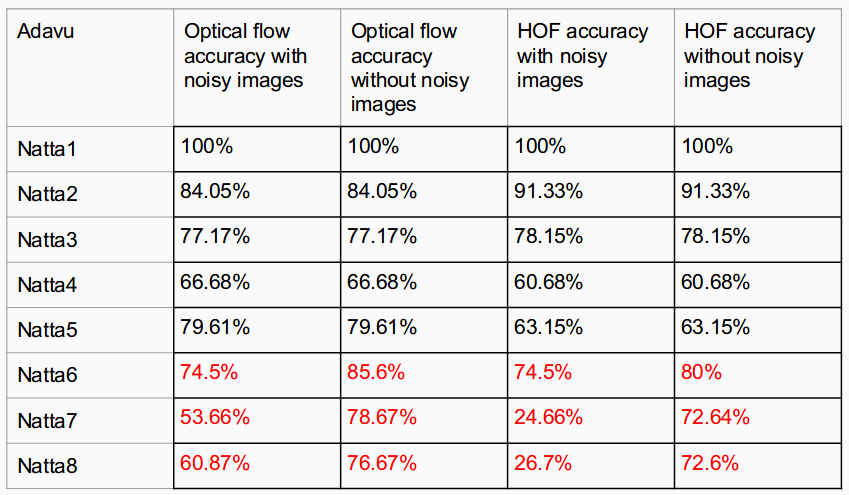
\includegraphics[width=120mm]{Pictures/res4.png}
\end{figure}


\section{Supervised Learning}

As we have seen dense optical flow as the better feature compared to HOF. we used dense optical flow for the feature extraction.But the problem is feature vector are of different sizes for different motions,we made all of them equal size by appending with a small value (1e-5).we then used SVM for classification.We have trained the svm on one performance of the dancer and tested on the other performance.

\subsection{SVM Results}

\begin{figure} [H]
\centering
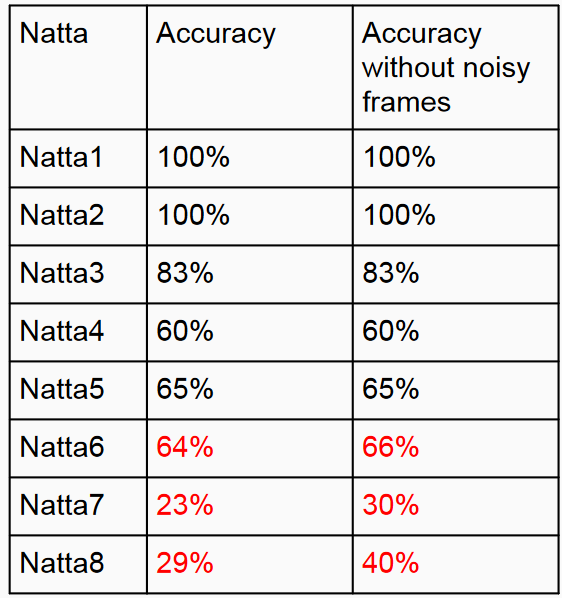
\includegraphics[width=80mm]{Pictures/res5.png}
\end{figure}

Here note that removing noisy motions doesn't increased accuracy much because noisy motions affect only the DTW Result.

\subsection{Approach 2 : K - Nearest Neighbour}

In this approach we have taken one performance of a dancer as training data and tested it on the other performance.For each motion in test data we assign it to the most similar motion in training set.The "most similar" is measured by Dense Optical Flow and DTW.

Here the removal of noisy frames had increased accuracy since here we used DTW and the noisy motions are effecting DTW result.

\begin{figure} [H]
\centering
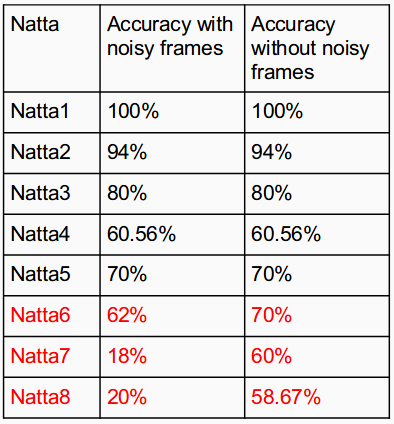
\includegraphics[width=80mm]{Pictures/KNN_res.png}
\end{figure}




\section{Conclusion \& Future Work }

In this work we tried  various approaches for clustering of motions.In the unsupervised approach, using dense optical flow we achieved an average accuracy of 81\% and by using HOF we achieved 77\% average accuracy.However using HOF decreased the running time of the algorithm by half since it decreases the feature vector size.we have also tried using SVM for classification but the accuracy was not so good.

In future,we want to automate the process to find optimal no of clusters in the video.we also wanted to extend this approach to skeletal videos.we aim to improve the SVM classification approach by training on more data.






 
%\input{Chapters/Chapter6} 
%\input{Chapters/Chapter7} 

%----------------------------------------------------------------------------------------
%	THESIS CONTENT - APPENDICES
%----------------------------------------------------------------------------------------

\addtocontents{toc}{\vspace{2em}} % Add a gap in the Contents, for aesthetics

\appendix % Cue to tell LaTeX that the following 'chapters' are Appendices

% Include the appendices of the thesis as separate files from the Appendices folder
% Uncomment the lines as you write the Appendices



\addtocontents{toc}{} % Add a gap in the Contents, for aesthetics

\backmatter

%----------------------------------------------------------------------------------------
%	BIBLIOGRAPHY
%----------------------------------------------------------------------------------------
%\nocite{*}
\label{Bibliography}

\lhead{\emph{Bibliography}} % Change the page header to say "Bibliography"
\begin{thebibliography}{999}

\bibitem{Aligned}
Feng Zhou, F. D. l. Torre and J. K. Hodgins, "Aligned Cluster Analysis for temporal segmentation of human motion," 2008 8th IEEE International Conference on Automatic Face \& Gesture Recognition, Amsterdam, 2008, pp. 1-7.
doi: 10.1109/AFGR.2008.4813468 \href{http://ieeexplore.ieee.org/stamp/stamp.jsp?tp=&arnumber=4813468&isnumber=4813301}{publisher}

\bibitem{MotionClustering}
Kexue Dai, Guohui Li and Defeng Wu, "Motion clustering for similar video segments mining," 2006 12th International Multi-Media Modelling Conference, Beijing, 2006, pp. 4 pp.-.
doi: 10.1109/MMMC.2006.1651368
\href{http://ieeexplore.ieee.org/stamp/stamp.jsp?tp=&arnumber=1651368&isnumber=34625}{publisher}

\bibitem{Spectral}
Hongbin Wang and Hua Lin, "A spectral clustering approach to motion segmentation based on motion trajectory," 2003 International Conference on Multimedia and Expo. ICME '03. Proceedings (Cat. No.03TH8698), Baltimore, MD, USA, 2003, pp. II-793.
doi: 10.1109/ICME.2003.1221736
\href{http://ieeexplore.ieee.org/stamp/stamp.jsp?tp=&arnumber=1221736&isnumber=27437}{publisher}

\bibitem{Spectral1}
von Luxburg, U. Stat Comput (2007) 17: 395. https://doi.org/10.1007/s11222-007-9033-z
\href{https://link.springer.com/content/pdf/10.1007%2Fs11222-007-9033-z.pdf}{publisher}

\bibitem{DTW}
FastDTW: Toward Accurate Dynamic Time Warping in 
Linear Time and Space
Stan Salvador and Philip Chan 
Dept. of Computer Sciences 
Florida Institute of Technology 
Melbourne, FL  32901 
\href{https://pdfs.semanticscholar.org/05a2/0cde15e172fc82f32774dd0cf4fe5827cad2.pdf}{publisher}

\bibitem{Optical}
Optical Flow Estimation
David J. Fleet, Yair Weiss
\href{http://www.cs.toronto.edu/~fleet/research/Papers/flowChapter05.pdf}{publisher}


\bibitem{}
A Tutorial to understand DTW
\href{http://mirlab.org/jang/books/dcpr/dpDtw.asp?title=8-4%20Dynamic%20Time%20Warping}{tutorial}







\end{thebibliography}

\end{document}  
